\section{Theory}
\subsection{The Classical Restricted Boltzmann Machine}
The Restricted Boltzmann Machine (RBM) is an energy-based model defined by the energy function~\cite{goodfellow_deep_learning}
\begin{align}
    E(\vec{v}, \vec{h})
        &= -\sum_i a_i v_i - \sum_j b_j h_j - \sum_{i,j} v_i w_{ij} h_j \label{eq:rbm_energy} \\
        &= -\vec{a}^\intercal\vec{v} - \vec{b}^\intercal\vec{h} - \vec{v}^\intercal\mat{W}\vec{h} \label{eq:rbm_energy_vectorized}
\end{align}
where
\begin{itemize}
    \item \( \vec{v} \in \binset^{n_v} \) represents the visible units, with associated bias vector \( \vec{a} \in \R^{n_v} \).
    \item \( \vec{h} \in \binset^{n_h} \) represents the hidden units, with associated bias vector \( \vec{b} \in \R^{n_h} \).
    \item \( \mat{W} \in \R^{n_v \times n_h} \) represents the weights corresponding to the interaction strengths between visible and hidden units.
\end{itemize}

\begin{figure}[!htb]
    \begin{center}
        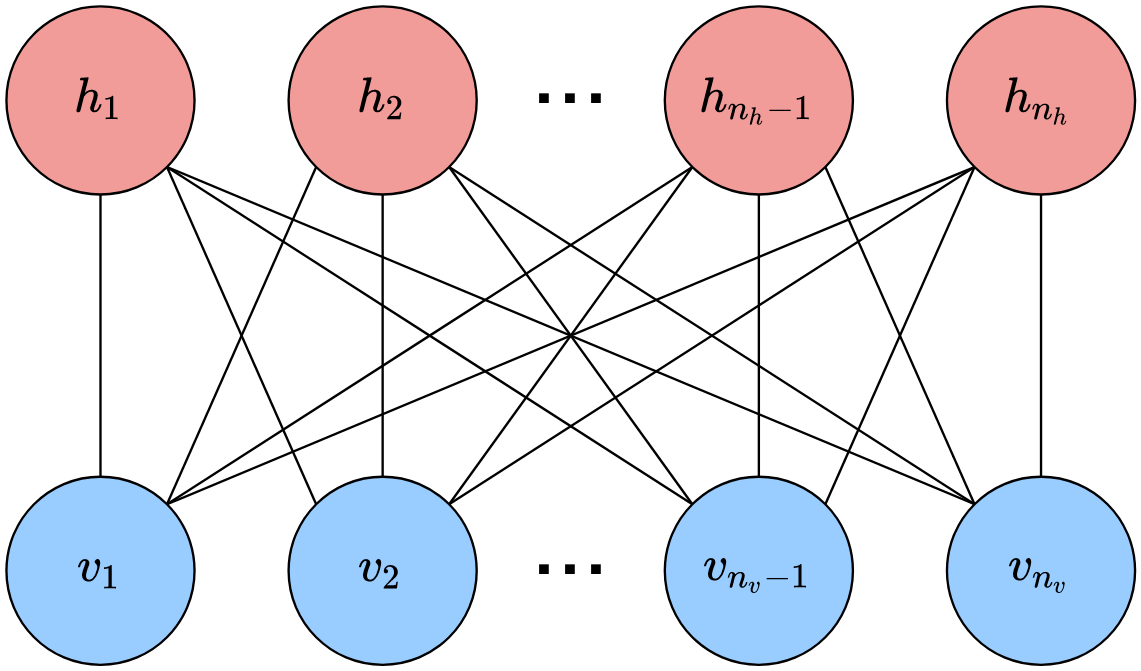
\includegraphics[width=1\linewidth]{rbm_diagram.png}
    \end{center}
    \caption{Diagram of a restricted Boltzmann machine with \( n_v \) visible units and \( n_h \) hidden units.}
    \label{fig:rbm_diagram}
\end{figure}

It is termed \textit{restricted} due to the fact that there are no intra-layer connections, i.e., visible units are only connected to hidden units, and vice versa.
An example diagram is depicted in~\cref{fig:rbm_diagram}.

The probability to find the system in the configuration \( \{\vec{v},\vec{h}\} \) is given by the Boltzmann distribution (with \( \beta = \frac{1}{k_BT} = 1 \))
\begin{align}
    p(\vec{v}, \vec{h}) = \frac{1}{Z} e^{-E(\vec{v},\vec{h})}
\end{align}
with intractable~\cite{long_servedio_2010} partition function
\begin{align}
    Z = \sum_{\vec{v},\vec{h}} e^{-E(\vec{v},\vec{h})}
\end{align}

The imposed restrictions on intra-layer connections enable us to write the conditional probabilities of the layers as the product of the individual units' probabilities~\footnote{Here \( \sigma(x) \) is the logistic sigmoid function and \( \odot \) denotes element-wise multiplication.} (see \cref{app:conditional_probabilities_derivation} for full derivation)
\begin{align}
    p(\vec{h} | \vec{v})
        &= \prod_j \sigma\big( (2\vec{h} - 1) \odot (\vec{b} + \mat{W}^\intercal\vec{v}) \big)_j \\
    p(\vec{v} | \vec{h})
        &= \prod_i \sigma\big( (2\vec{v} - 1) \odot (\vec{a} + \mat{W}\vec{h}) \big)_i
\end{align}

\subsection{Optimizing an RBM}
Due to the intractability of the partition function, the model cannot be solved exactly, thus we resort to other methods to optimize it such as likelihood maximization via gradient descent.
For data distribution \( p_\text{data} \) and parameters \( \theta = (\mat{W}, \vec{a}, \vec{b}) \) the average log-likelihood is given by
\begin{align}
    \ell(\theta) = \sum_{\vec{v}} p_{\text{data}}(\vec{v}) \log \frac{1}{Z} \sum_\vec{h} e^{-E(\vec{v},\vec{h})}
\end{align}
with gradients (see \cref{app:rbm_log_likelihood_derivation} for full derivation)
\begin{align}
    \partial_{w_{ij}} \ell(\theta)
        &= \langle v_i h_j \rangle_{\text{data}} - \langle v_i h_j \rangle_{\text{model}} \\
    \partial_{a_i} \ell(\theta)
        &= \langle v_i \rangle_{\text{data}} - \langle v_i \rangle_{\text{model}} \\
    \partial_{b_j} \ell(\theta)
        &= \langle h_j \rangle_{\text{data}} - \langle h_j \rangle_{\text{model}}
\end{align}
Therefore, the parameters at step \( t \) are given by
\begin{align}
    \mat{W}^{(t)}
        &= \mat{W}^{(t-1)} + \eta(\langle \vec{v} \vec{h}^\intercal \rangle_{\text{data}} - \langle \vec{v} \vec{h}^\intercal \rangle_{\text{model}}) \\
    \vec{a}^{(t)}
        &= \vec{a}^{(t-1)} + \eta(\langle \vec{v} \rangle_{\text{data}} - \langle \vec{v} \rangle_{\text{model}}) \\
    \vec{b}^{(t)}
        &= \vec{b}^{(t-1)} + \eta(\langle \vec{h} \rangle_{\text{data}} - \langle \vec{h} \rangle_{\text{model}})
\end{align}
where \( \eta \) is the learning rate hyperparameter.

Since \( p(\vec{v}) \) can not be sampled directly, it must be sampled using a Markov chain Monte Carlo (MCMC) method.
The way to do so is through Gibbs sampling~\cite{hinton_rbm_training}, which uses the conditional probabilities \( p(\vec{h}|\vec{v}) \) and \( p(\vec{v}|\vec{h}) \).
One starts with a visible vector and then samples the hidden units conditioned on the visible, followed by sampling the visible conditioned on the hidden, and so forth until a desired thermalization threshold is reached.
How many steps it requires to reach thermalization is model dependent and can be estimated by analyzing the autocorrelations of a Markov chain generated by the model.
The algorithm for Gibbs sampling is given in \cref{alg:Gibbs} and illustrated in \cref{fig:gibbs_sampling_diagram}.
For brevity the algorithm is presented in a vectorized format.

\begin{algorithm}
\caption{Gibbs Sampling}
\begin{algorithmic}[1]
    \Procedure{Gibbs}{$\vec{v},n,\mat{W},\vec{a},\vec{b}$}
        \State $n_v \gets$ length$(\vec{a})$
        \State $n_h \gets$ length$(\vec{b})$
        \For{$k$ in 1 to $n$}
            \State $\vec{r} \sim$ Uniform$(0, 1, n_h)$
            \State $\vec{h} \gets \vec{r} < \sigma(\vec{b} + \mat{W}^\intercal\vec{v})$
                \Comment $\sigma, <$ applied element-wise
            \State $\vec{r} \sim$ Uniform$(0, 1, n_v)$
            \State $\vec{v} \gets \vec{r} < \sigma(\vec{a} + \mat{W}\vec{h})$
                \Comment $\sigma, <$ applied element-wise
        \EndFor
        \State \Return $\vec{v}$
    \EndProcedure
\end{algorithmic}
\label{alg:Gibbs}
\end{algorithm}
The Uniform$(a, b, n)$ function in \cref{alg:Gibbs} produces a length \( n \) vector of uniform i.i.d. random variables on the interval $[a, b)$.

\begin{figure}
    \begin{center}
        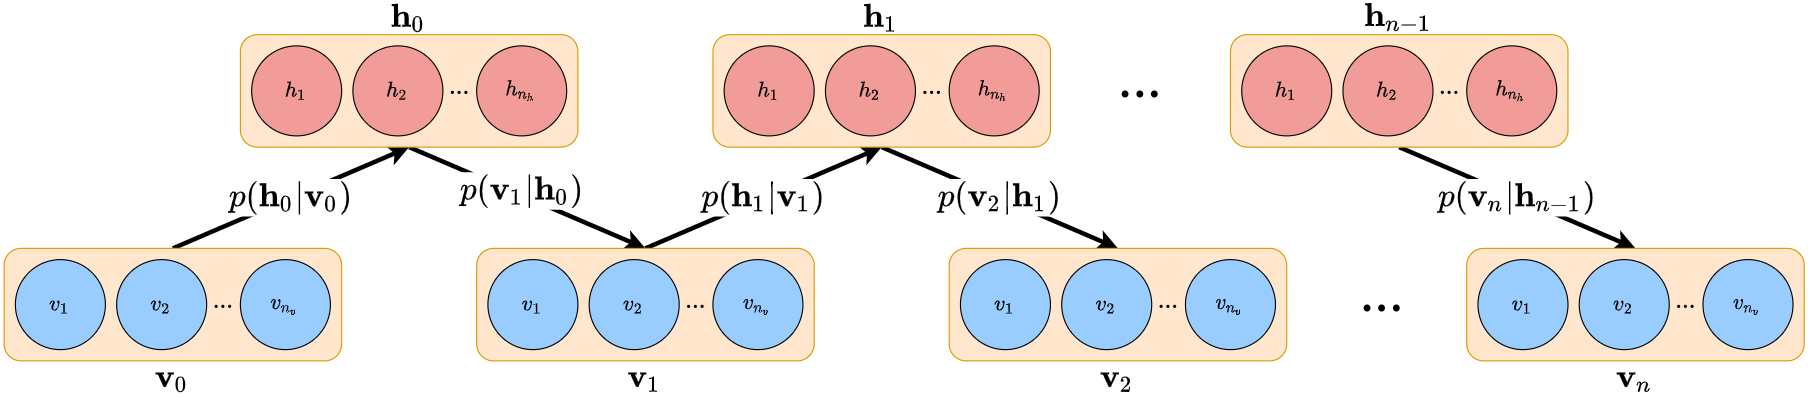
\includegraphics[width=1\linewidth]{gibbs_sampling_diagram.png}
    \end{center}
    \caption{Illustration of the Gibbs sampling procedure.}
    \label{fig:gibbs_sampling_diagram}
\end{figure}

The standard procedure for training an RBM is called \( n \)-step contrastive divergence (CD-\( n \)), with \( n \) often taken to be one in practice~\cite{hinton_rbm_training}.
The algorithm is detailed in \cref{alg:CDn}, where one can see that \( n \) corresponds to how many Gibbs sampling steps are between the positive and negative phase gradients.
Applying the algorithm to a mini-batch is essentially the same except that one divides the learning rate by the size of the mini-batch to get a mini-batch averaged gradient.

\begin{algorithm}
    \caption{$n$-Step Contrastive Divergence (CD-$n$)}
\begin{algorithmic}[1]
    \Procedure{CD}{$\vec{v}_+,n,\mat{W},\vec{a},\vec{b},\eta$}
        \Comment $\vec{v}_+$ is a training example
        \State $\vec{h}_+ \gets \sigma(\vec{b} + \mat{W}^\intercal\vec{v}_+)$
            \Comment $\sigma$ applied element-wise
        \State $\vec{v}_- \gets$ Gibbs$(\vec{v}_+,n,\mat{W},\vec{a},\vec{b})$
        \State $\vec{h}_- \gets \sigma(\vec{b} + \mat{W}^\intercal\vec{v}_-)$
            \Comment $\sigma$ applied element-wise
        \State $\mat{W} \gets \mat{W} + \eta(\vec{v}_+ \vec{h}_+^\intercal - \vec{v}_- \vec{h}_-^\intercal)$
        \State $\vec{a} \gets \vec{a} + \eta(\vec{v}_+ - \vec{v}_-)$
        \State $\vec{b} \gets \vec{b} + \eta(\vec{h}_+ - \vec{h}_-)$
        \State \Return $\mat{W}, \vec{a}, \vec{b}$
    \EndProcedure
\end{algorithmic}
\label{alg:CDn}
\end{algorithm}


\section{Application \& Results}
In the 2019 paper titled \textit{The Market Generator}~\cite{kondratyev_2019}, Kondratyev and Schwarz analyzed how an RBM could be used as a generative model to produce synthetic market data.
Specifically, they studied how it performed on the log returns of forex data for the same currencies as we analyze here for the time period 1999-2019.
They successfully showed that the RBM was able produce better results than the parametric model it was being compared to, and that in general the RBM is able to perform quite well as a regularized autoencoder that can generate samples from arbitrary probability distributions that it is trained on.

The framework they laid out to analyze their results is quite extensive, using a number of different metrics to evaluate how well the model can capture the intricacies of the data.
In this section we will analyze a lot of the same metrics so that we can verify our model achieves similar performance to theirs, as well as give us a framework to later compare the quantum model with.

\subsection{Models}
We will compare four different RBM models trained on the data laid out in the previous chapter, denoted by:
\begin{itemize}
    \item (B): trained on the base dataset.
    \item (V): trained on the base dataset with additional volatility indicators.
    \item (X): trained on the transformed dataset.
    \item (XV): trained on the transformed dataset with additional volatility indicators.
\end{itemize}
The models trained here use 64 (68 for ones with volatility indicators) visible units and 30 hidden units (the same as in~\cite{kondratyev_2019}), a batch size of 10, and an initial learning rate of \( 10^{-3} \) which decays by a factor of half every 1000 epochs after epoch 5000.
Models are based on scikit-learn's~\cite{python_sklearn} BernoulliRBM class.
Scikit-learn was forked~\footnote{https://github.com/cameronperot/scikit-learn/} to implement the ability to use a learning rate schedule with the BernoulliRBM class.

One of the drawbacks of the RBM is that it's not easy to track the training progress for our use case, as we found that the pseudolikelihood metric used by the scikit-learn package was not necessarily a good proxy for model performance.
The idea of tracking a quantity such as the KL divergence (as we do in the quantum Boltzmann machine chapter) was considered, but due to the high number of epochs and the thermalization requirements of samples generated by the RBM, this is not very feasible as the training time would increase significantly.
Therefore, we will only analyze the final results of the model.
To this end, we generated an ensemble of 100 sample sets, each having the same number of samples as the number of training examples in the dataset.

\subsection{Model Results}
\subsubsection{Marginal Distributions}
The first thing we wish to look at is how well the model was able to learn the marginal distributions.
For this we examine the KL divergences of the marginal distributions of each currency pair in~\cref{tbl:rbm_KL_divergences}.
Here we see that all models learned to reproduce the marginal distributions quite well, but the models using the transformed datasets perform slightly better.
We also notice that the models trained on the non-transformed datasets have a harder time with the USDCAD marginal.
The performance of the models on the marginal distributions is also visualized with QQ plots in~\cref{fig:rbm_qq_plots}
\begin{table}[!htb]
    \centering
    \begin{adjustbox}{max width=\textwidth}
        \input{../tables/rbm/kl_divergences.tbl}
    \end{adjustbox}
    \caption{KL divergences of the RBM models. All numbers are shown in the format average \(\pm\) one standard deviation from an ensemble of size 100. We note that this is an approximation to the true KL divergence, as here we use a histogram approach with 32 bins.}
    \label{tbl:rbm_KL_divergences}
\end{table}
\begin{figure}[!htb]
    \begin{center}
        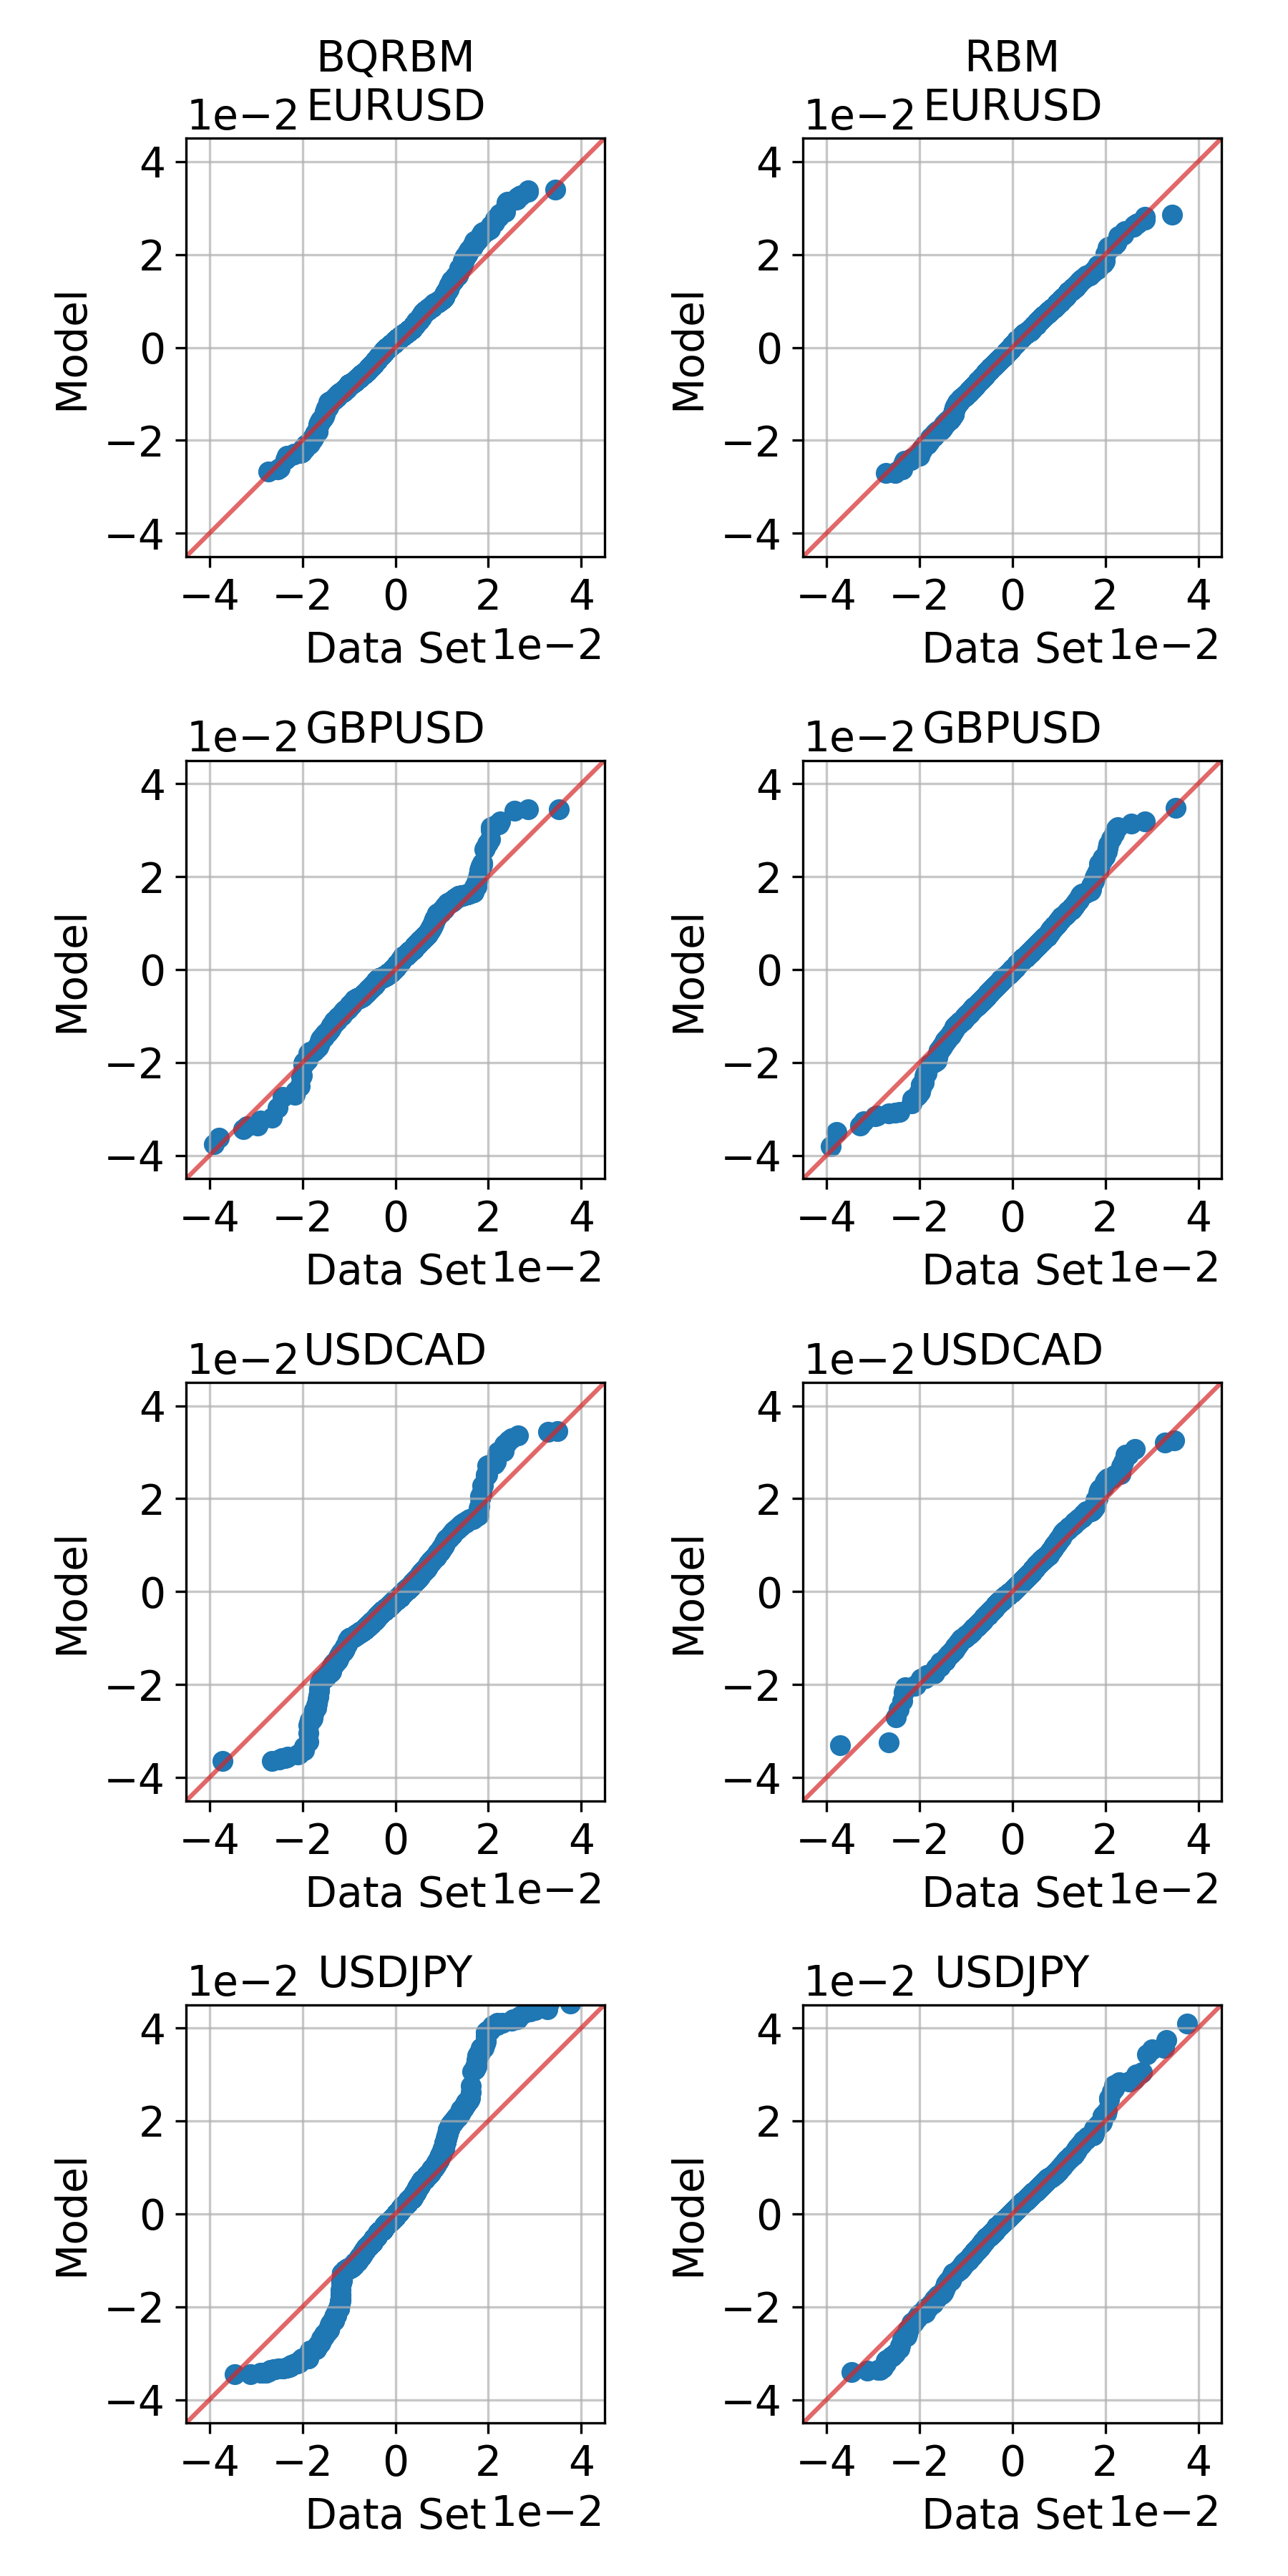
\includegraphics[width=1\linewidth]{rbm/qq.png}
    \end{center}
    \caption{QQ plots of the RBM models. Note that this is only one instance of samples from the ensemble, and is not entirely representative of the models' performance.}
    \label{fig:rbm_qq_plots}
\end{figure}

\subsubsection{Correlations}
The distribution is in a sense more than just the sum of the parts.
Beyond learning the marginal distributions, we need the model to capture the correlations between the currency pairs.

Next we analyze the correlation coefficients in~\cref{tbl:rbm_correlation_coefficients} to see how well the models learned the correlations between the currency pairs.
Again we see that the generated data is able to reproduce the structure of the correlation coefficients reasonably well, with the models trained on the transformed data performing better.
Details on how the correlation coefficients are computed and how to interpret them can be found in~\cref{app:correlation_coefficients}.
\begin{table}[!htb]
    \centering
    \begin{adjustbox}{max width=\textwidth}
        \input{../tables/rbm/correlation_coefficients.tbl}
    \end{adjustbox}
    \caption{Correlation coefficients of the data vs. samples generated by the RBM models. The RBM numbers are shown in the format average \(\pm\) one standard deviation from an ensemble of size 100.}
    \label{tbl:rbm_correlation_coefficients}
\end{table}

\subsubsection{Volatilities}
Examining the historical volatilities in~\cref{tbl:rbm_volatilities} continues to push the narrative that the RBMs are learning the intricacies of the data.
We see that the models are able to reproduce similar volatility structures, albeit marginally higher than that of the data.
\begin{table}[!htb]
    \centering
    \begin{adjustbox}{max width=\textwidth}
        \input{../tables/rbm/volatilities.tbl}
    \end{adjustbox}
    \caption{Historical volatilities of the data vs. samples generated by the RBM models. All numbers are shown in the format average \(\pm\) one standard deviation from an ensemble of size 100.}
    \label{tbl:rbm_volatilities}
\end{table}

\subsubsection{Tails}
One of the most important things that we require the model to learn is the tail events, as these play a crucial role in financial risk management.
The models trained on the transformed data seem to learn the lower tails a little bit better for most currency pairs, but overestimate the upper tail of EURUSD.
It's hard to say overall if one model performs better than another here.
\begin{table}[!htb]
    \centering
    \begin{adjustbox}{max width=\textwidth}
        \input{../tables/rbm/tails.tbl}
    \end{adjustbox}
    \caption{Lower and upper tails, i.e., 1st and 99th percentiles, of the data vs. samples generated by the RBM models. All numbers are shown in the format average \(\pm\) one standard deviation from an ensemble of size 100.}
    \label{tbl:rbm_tails}
\end{table}

We also studied the tail concentration functions (see~\cref{app:tail_concentration_functions} for definitions and interpretations) between currency pairs in~\cref{fig:rbm_tail_concentrations}.
Here we noticed that all models perform exceptionally well for the most part outside of a few minor regions in the EURUSD/GBPUSD, EURUSD/USDJPY, and GBPUSD/USDJPY plots.
The differences aren't so stark here between the RBM models, but when Kondratyev and Schwarz performed the same comparison to the parametric model it was clear that the RBM was the better performer.
\begin{figure}[!htb]
    \begin{center}
        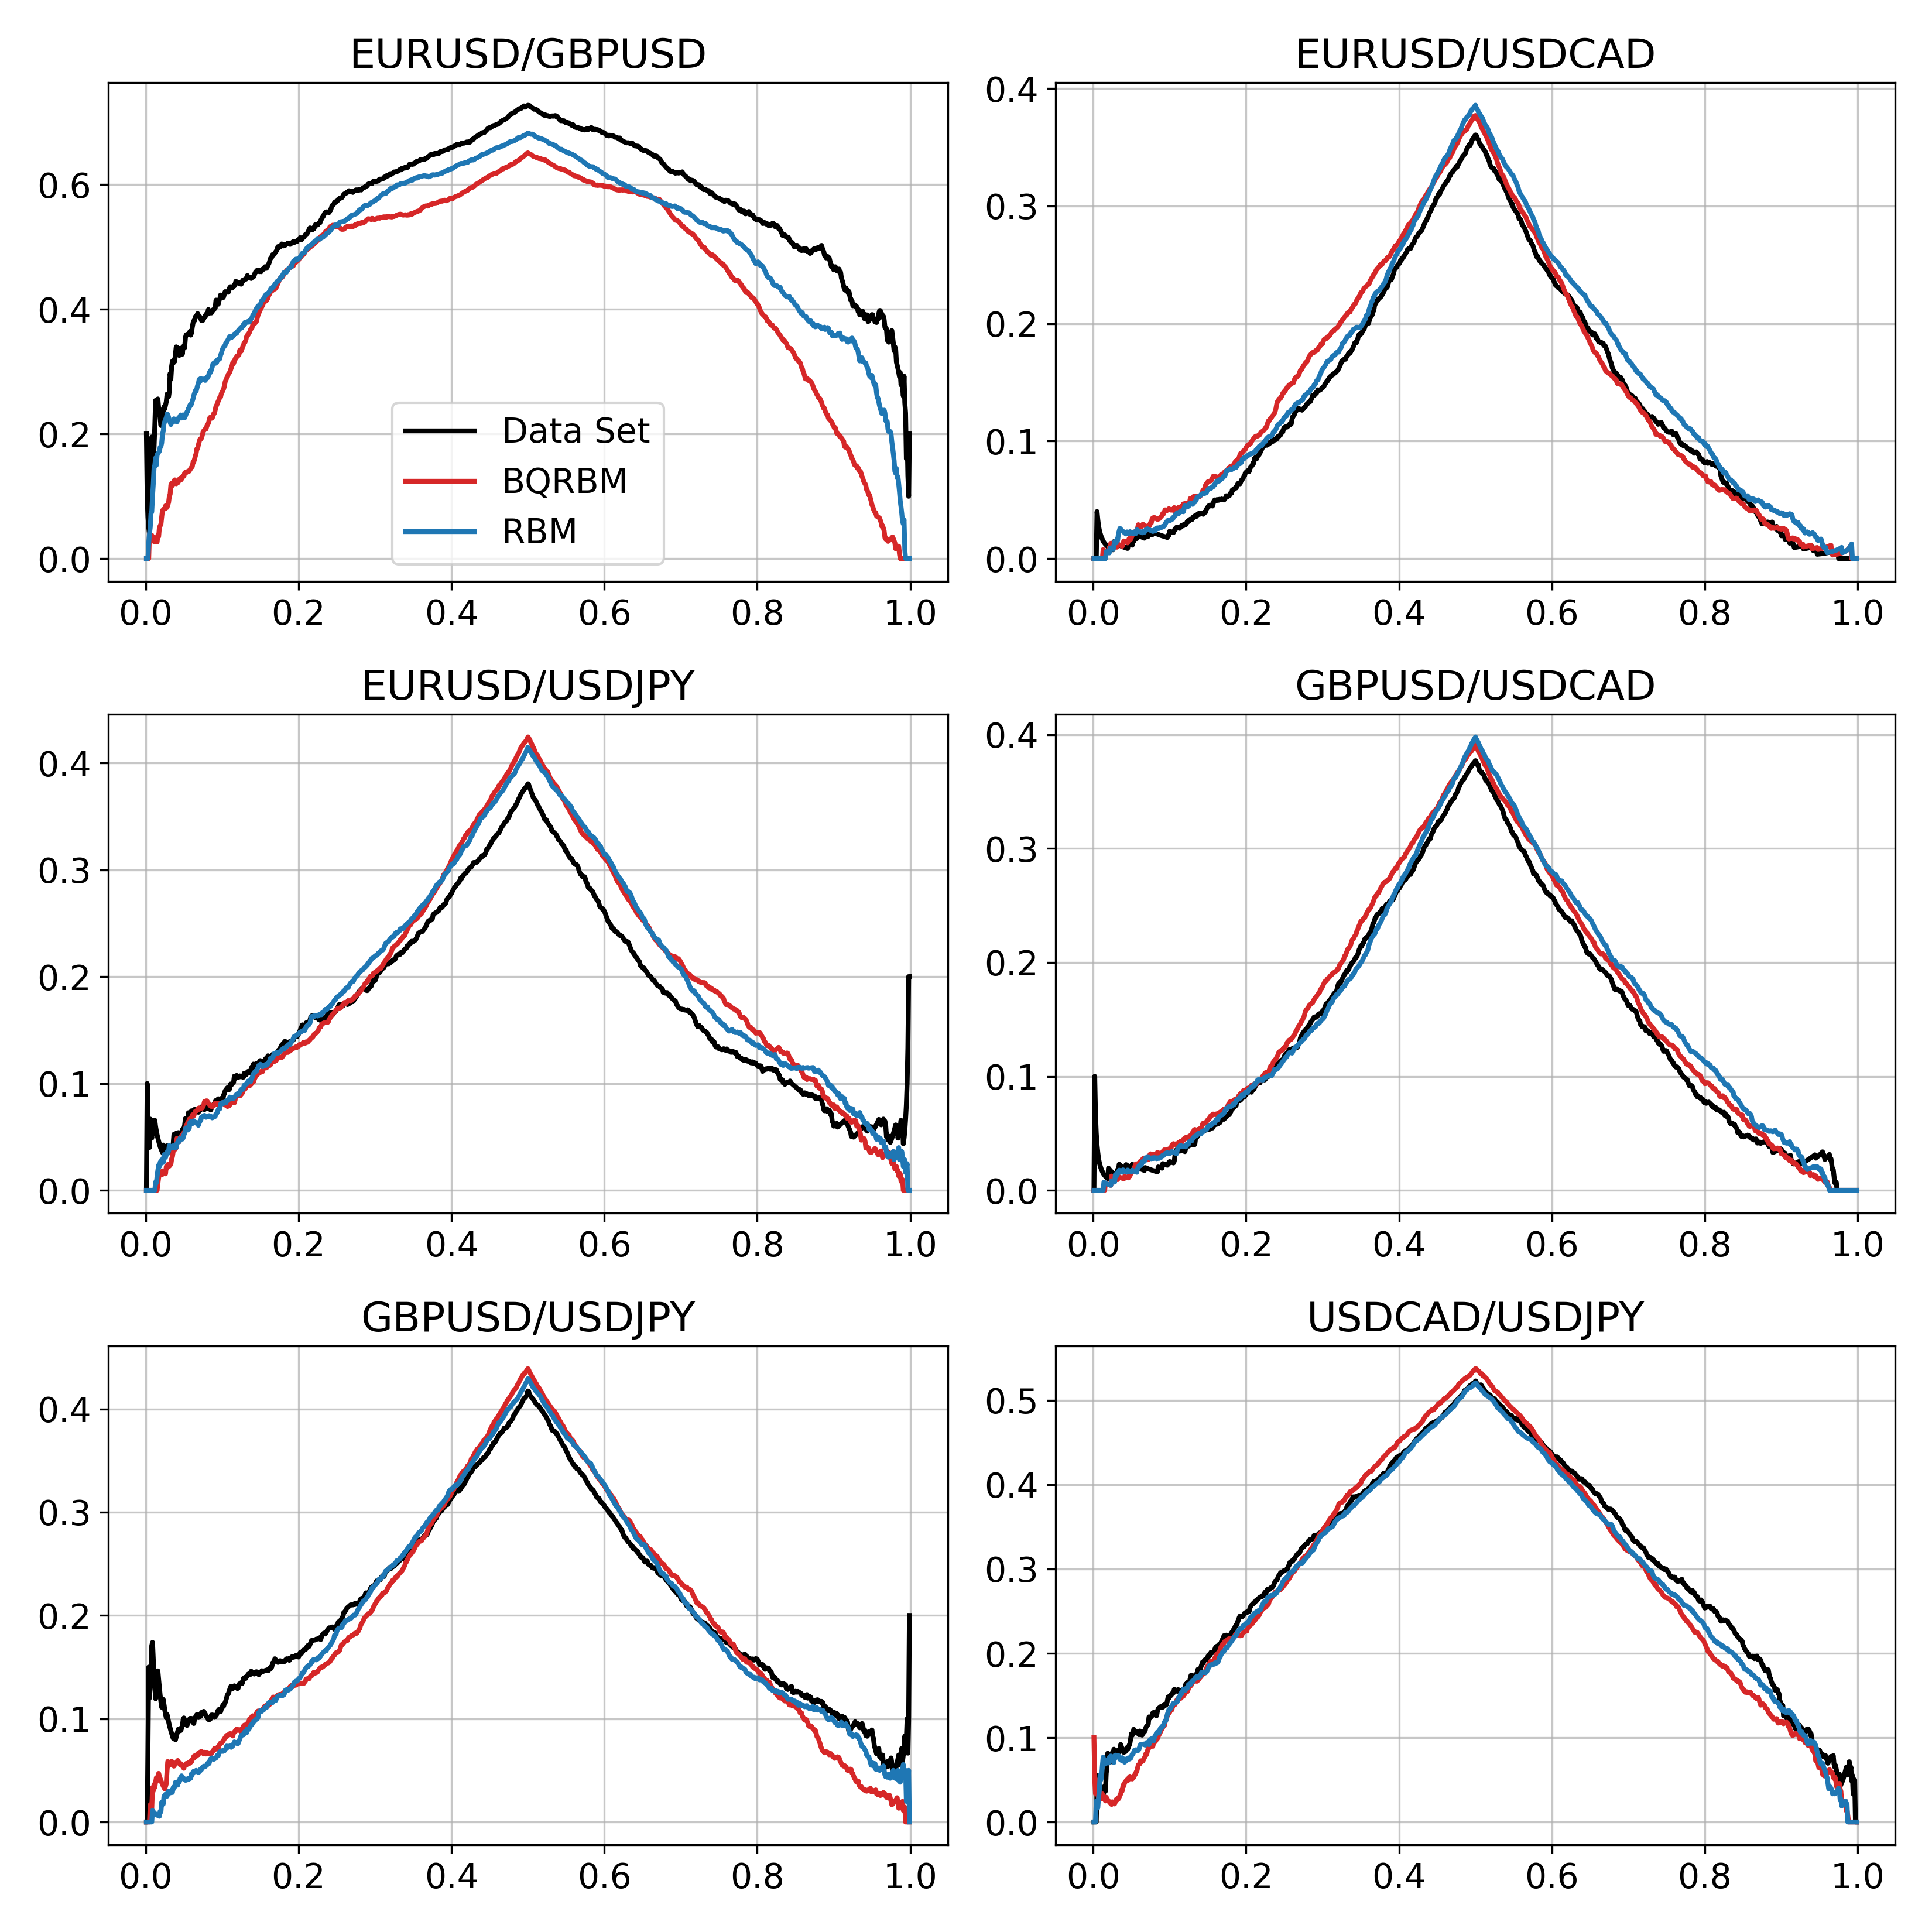
\includegraphics[width=1\linewidth]{rbm/tail_concentrations.png}
    \end{center}
    \caption{Tail concentration functions of the data vs. samples generated by the RBM models.}
    \label{fig:rbm_tail_concentrations}
\end{figure}

\subsubsection{Conditional Sampling}
One of the advantages of the RBM is the ability to perform conditional sampling.
For the datasets with additional volatility indicators, we have the ability to condition on these indicators to sample from a specific volatility regime.
This is useful for example if we are trying to generate real-world data that fits the current volatility landscape.

This leads us to look at the conditional volatilities, i.e., seeing how well the model can reproduce the volatilities from the two volatility regimes.
Laid out in~\cref{tbl:rbm_conditional_volatilities}, we see that the RBMs produce samples with slightly (higher) lower volatilities in the (low) high regime, but overall pretty much in agreement with the data.
\begin{table}[!htb]
    \centering
    \begin{adjustbox}{max width=\textwidth}
        \input{../tables/rbm/conditional_volatilities.tbl}
    \end{adjustbox}
    \caption{Conditional historical volatilities of the data vs. samples generated by the RBM models. All numbers are shown in the format average \(\pm\) one standard deviation from an ensemble of size 100.}
    \label{tbl:rbm_conditional_volatilities}
\end{table}

\subsubsection{Autocorrelations}
As mentioned before, the classical RBM requires more computational resources to produce good samples because of thermalization requirements.
Therefore, we must examine the autocorrelations to see how dependent samples are on the previous, so that we can get an idea of how many Gibbs steps we need between samples to consider them statistically independent.
More information about the autocorrelation function and time can be found in~\cref{app:autocorrelation_analysis}.

In~\cref{fig:rbm_autocorrelation_functions} we see the 1-day lag autocorrelation functions plotted for the various models and currency pairs.
From first observation we see the autocorrelations fall off much sooner for the models trained on the transformed datasets for all currency pairs.
This observation is confirmed when looking at the estimated integrated autocorrelation times in~\cref{tbl:rbm_ac_times}.

It is not immediately clear why the transformed data leads to such shorter integrated autocorrelation times, but this is a welcomed trend as it means that less sampling steps are required to reach thermalization.
\begin{figure}[!htb]
    \begin{center}
        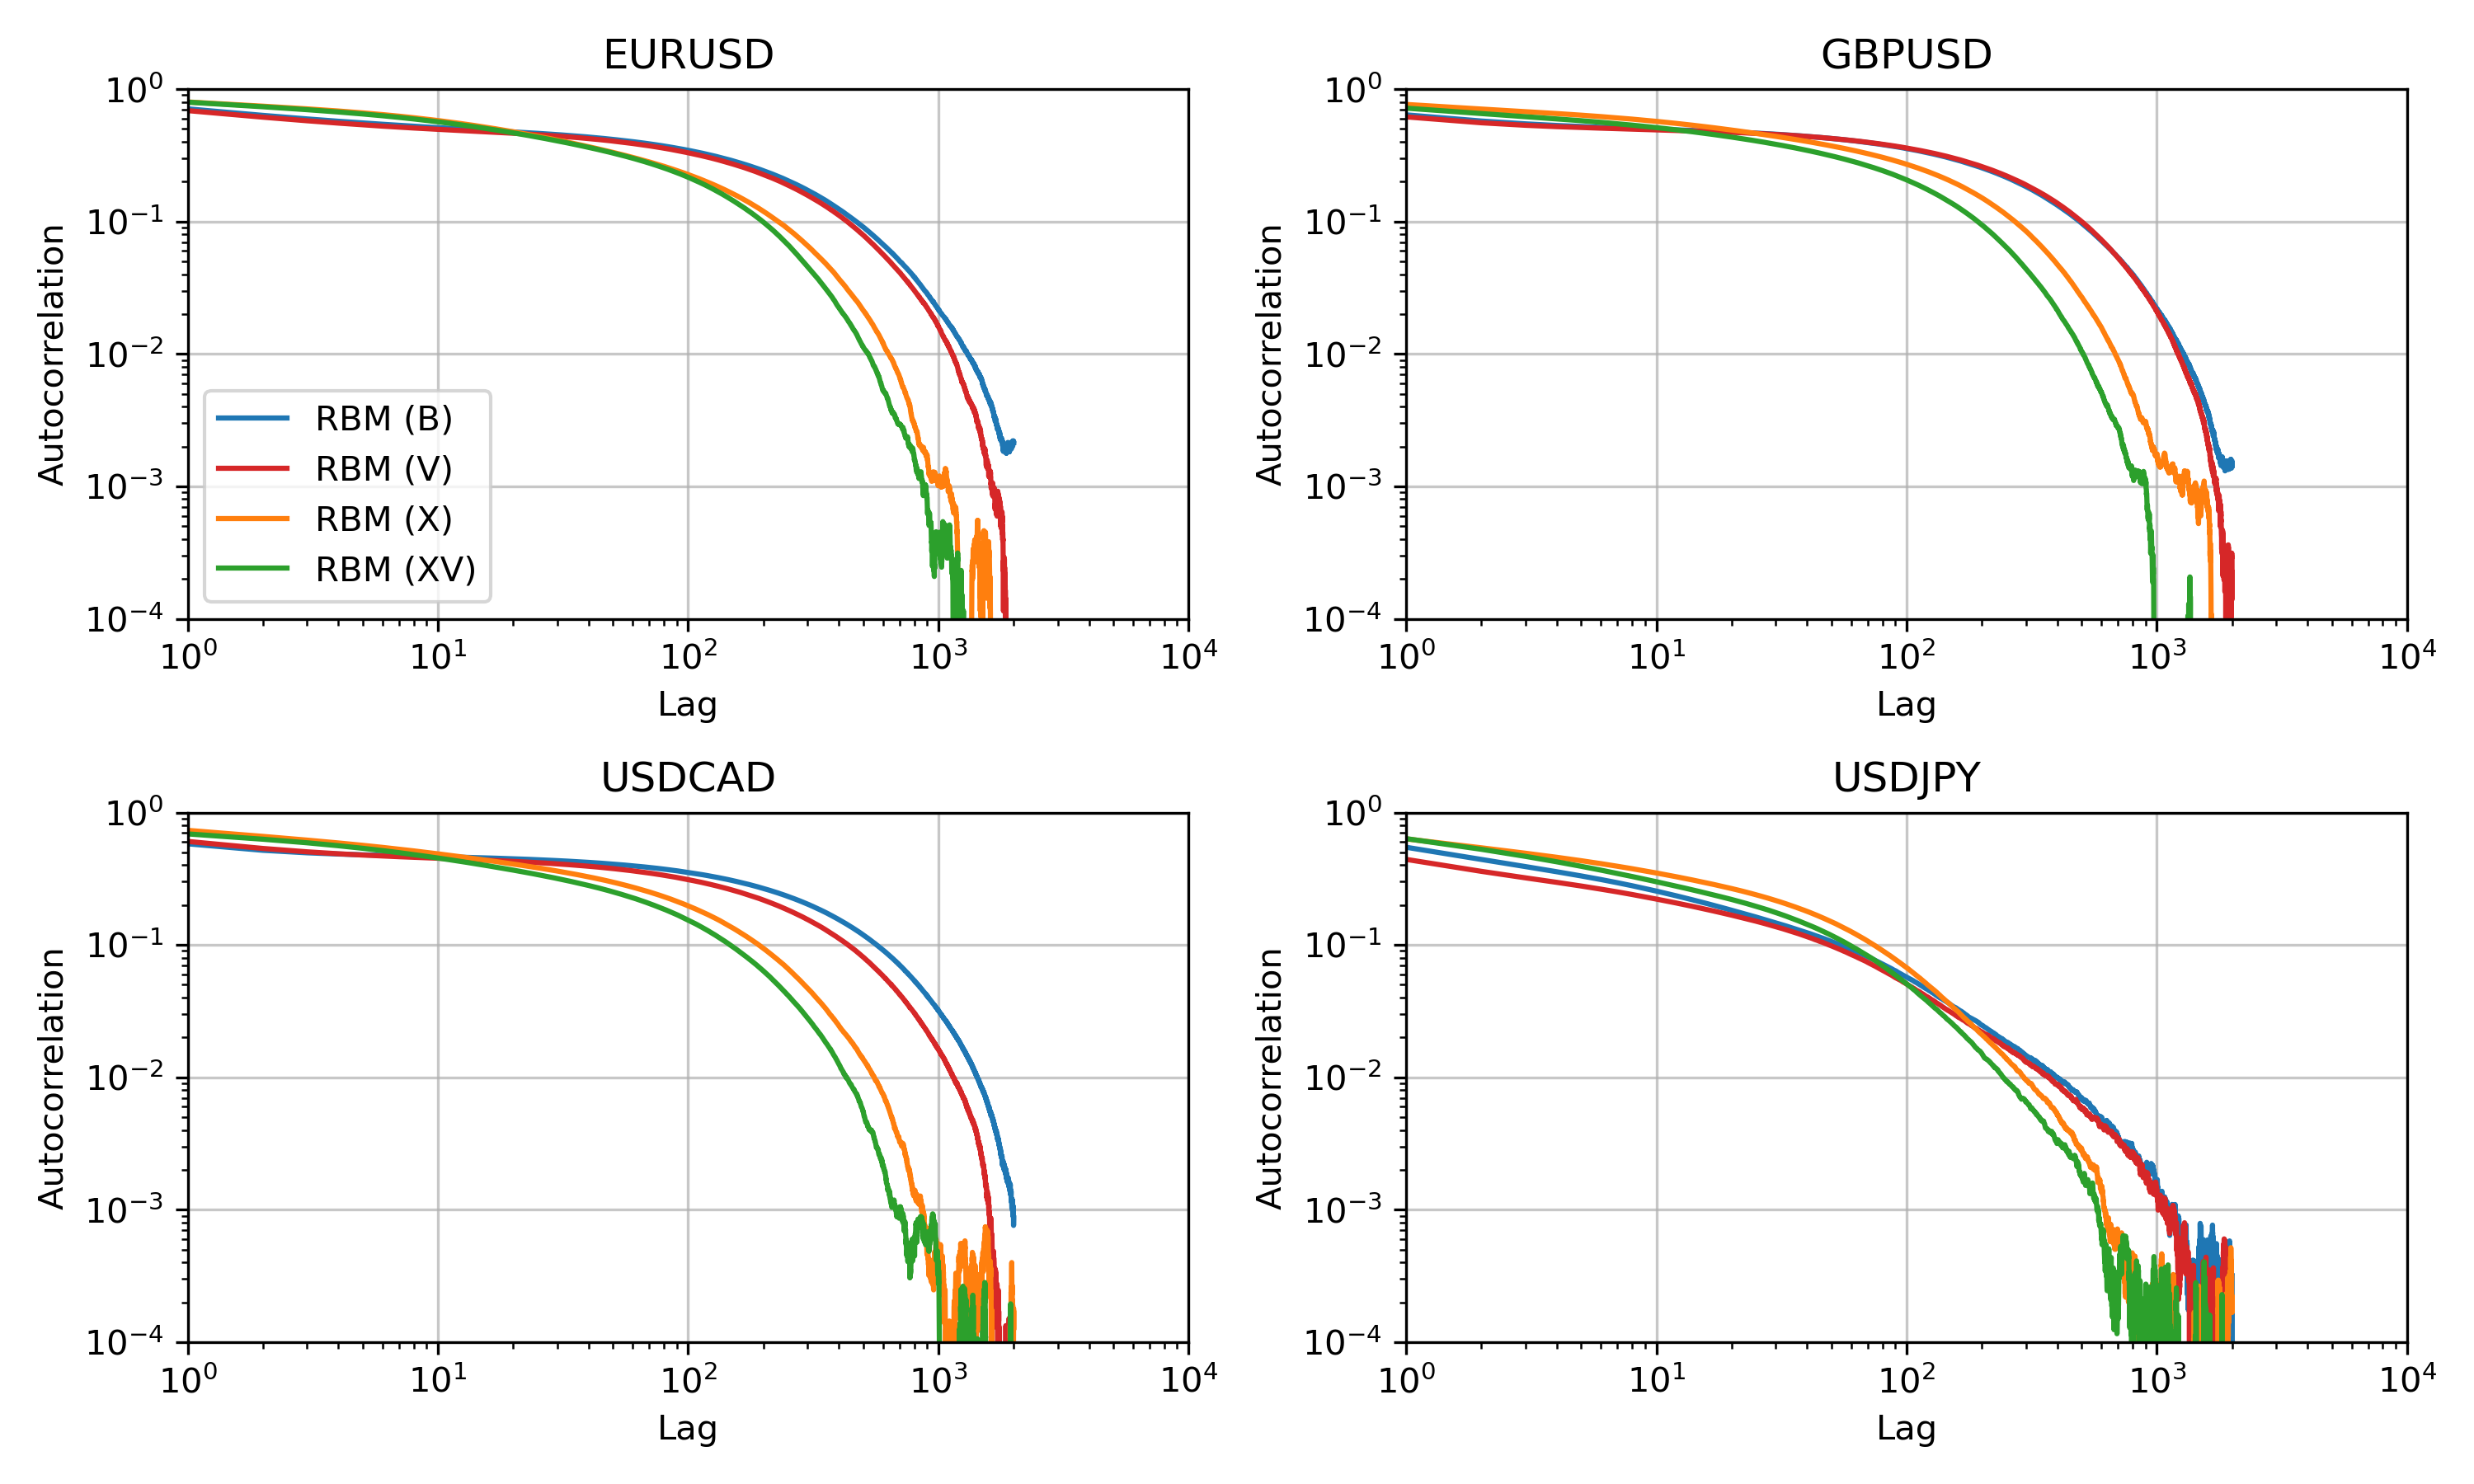
\includegraphics[width=1\linewidth]{rbm/autocorrelation_functions.png}
    \end{center}
    \caption{Autocorrelation functions of the RBM models indicate that the models trained on the transformed datasets thermalize faster. Function values are computed from Gibbs sample chains of length \( 10^8 \).}
    \label{fig:rbm_autocorrelation_functions}
\end{figure}
\begin{table}[!htb]
    \centering
    \begin{adjustbox}{max width=\textwidth}
        \input{../tables/rbm/autocorrelation_times.tbl}
    \end{adjustbox}
    \caption{Integrated autocorrelation times of the RBM models.}
    \label{tbl:rbm_ac_times}
\end{table}

\subsection{Summary}
The results in this section are in line with those obtained by Kondratyev and Schwarz in~\cite{kondratyev_2019}, and the differences are likely accounted for by the different dataset used in training, model hyperparameters, and the stochastic nature of the models.
This further confirms that the RBM is performant and can be used to generate samples from distributions with intricate structures, such as the correlations and volatilities seen here.

Overall it is difficult to say that one of the models performed the best, but the results of the models trained on the transformed data do offer hope that the results can be further improved by more advanced data preprocessing.
We do not investigate these possibilities any further though, given that this is not the main scope of this report.
The results in this section are mostly to act as a point of reference so that we have something to compare to when we train the quantum models.
